\label{chap:main_work}
In this chapter, the main contents of the thesis work are represented.
Figure \ref{fig:framework} shows the framework of the memory power
optimization process using the simulated annealing algorithm.
There are two kinds of input for the simulated annealing algorithm.
One is the input data related to the optimization problem.
These raw data is recorded in different text files but their data
structure is not suitable for the simulate annealing algorithm.
Thus, a proper input data organization is defined and a parsing
method is used to transform the raw data into this data organization.
Section \ref{sec:input_organ} discusses the input data organization
and the parsing method in detail.
The other kind of input for the algorithm is the algorithm parameter.
The discussion of these parameters are made in Section.....which also
introduce the design of the simulated in detail.
\begin{figure}[H]
	\begin{center}
		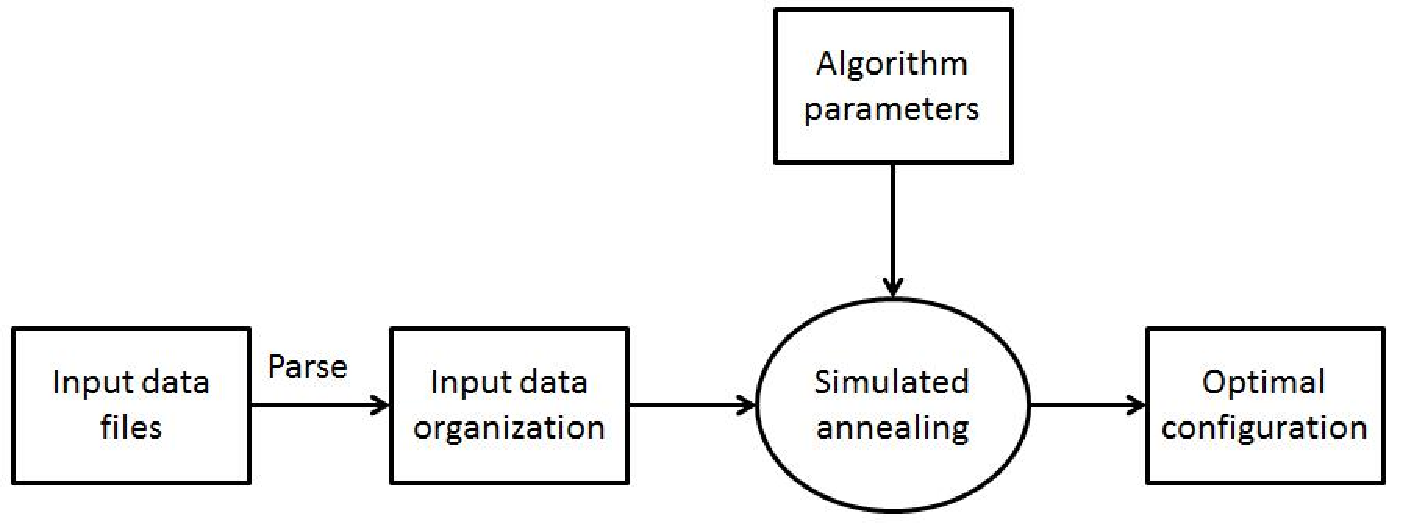
\includegraphics[width=0.7\textwidth]{optim_framework}
		\caption{Framework of The Simulated Annealing for Memory Power Optimization}
		\label{fig:framework}
	\end{center}
\end{figure}
	\section{Input data organization}
	\label{sec:input_organ}
	As discussed in Section \ref{sec:memory_partition}, the formal
	power model requires the parameters that are relevant to the
	memory types, the application profiles and the interconnect.
	Thus, these parameters are the input data to the simulated
	annealing algorithm.
	Since the object oriented programming is planned to be used for
	the implementation of the simulated annealing, the parameters
	that are related to the same item can be grouped together into
	one class. For example, the physical parameters that are
	relevant to the memory type can reside in the memory class.
	Figure \ref{fig:uml} shows the input parameters
	organization in the form of the UML class diagram.

	\begin{figure}[htb]
		\begin{center}
			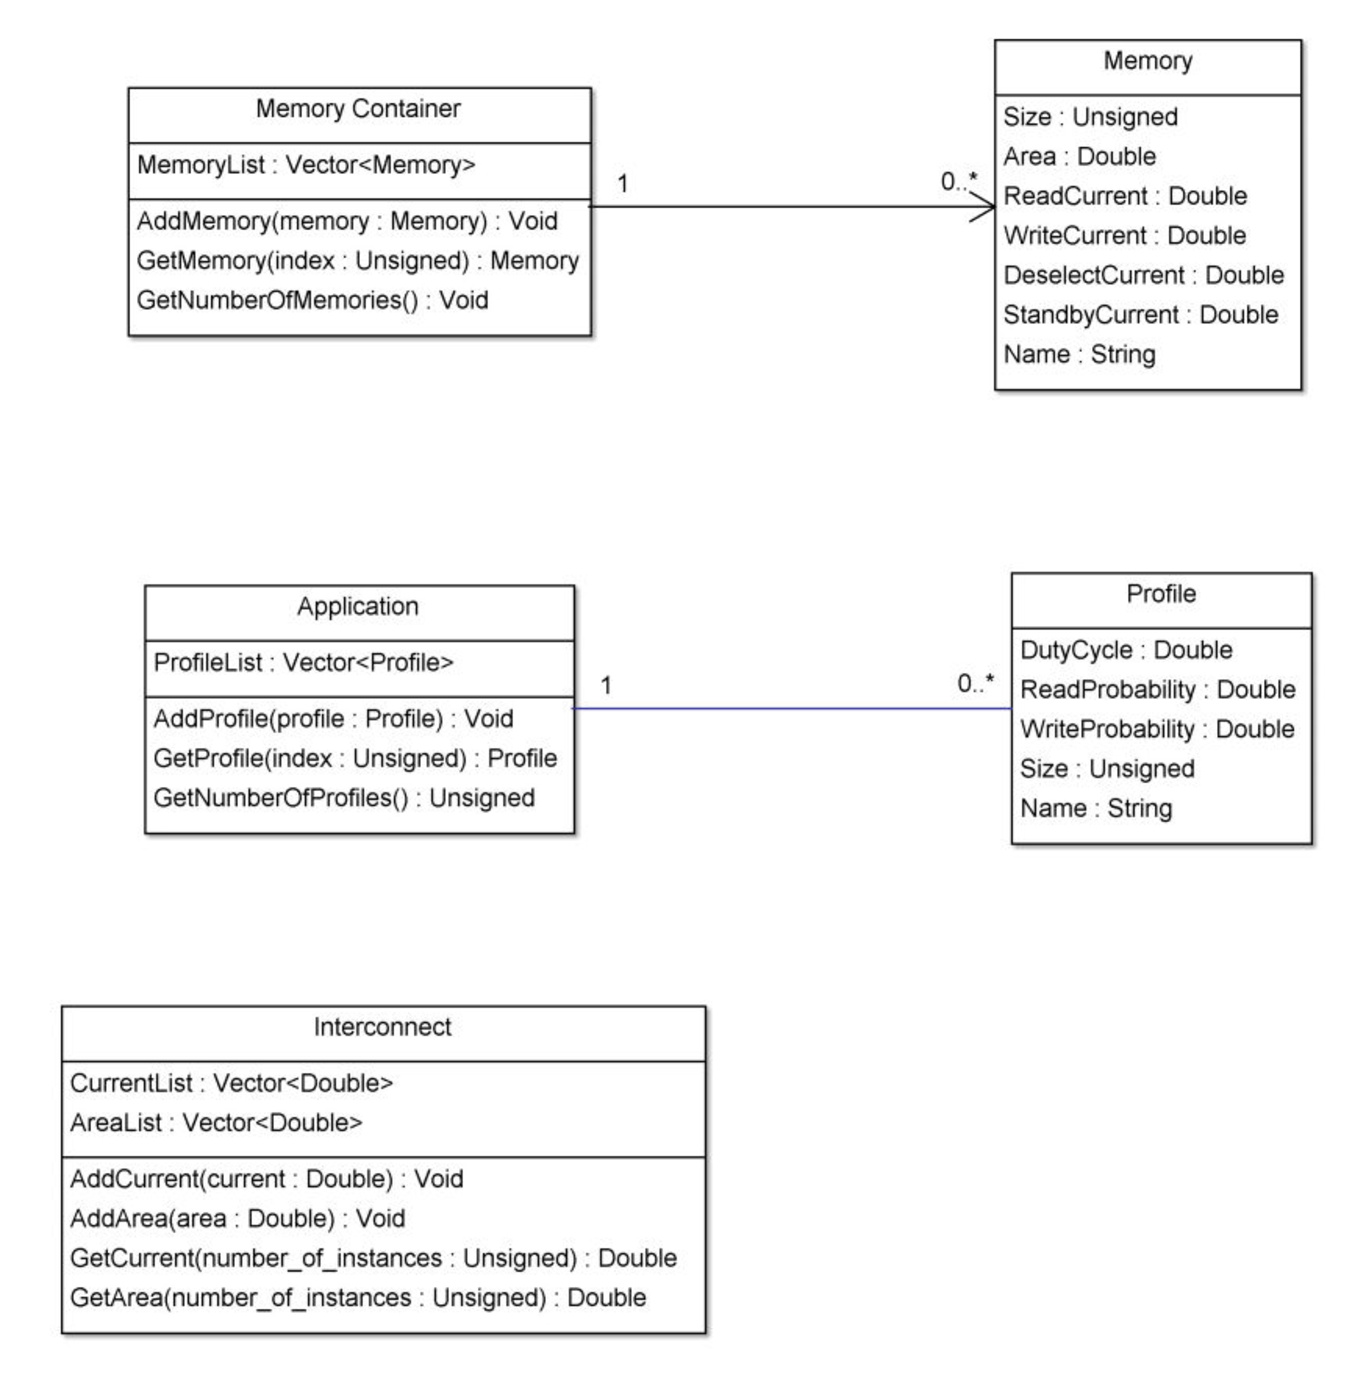
\includegraphics[width=0.7\textwidth]{uml_class}
			\caption{Input Parameter Organization in UML Diagram}
			\label{fig:uml}
		\end{center}
	\end{figure}
	
	The memory class includes all its parameters that are used in the
	formal power model.  Since there are a set of memory types in the
	power model, a set of objects of the memory class will be created in
	the simulated annealing algorithm as well. Thus the memory container
	class is defined to store these memory objects.
	And the algorithm can also retrieve the required objects and the
	total number of memory objects through the corresponding operations
	in the memory container class.
	The profile class and the application class are defined similarly
	to the memory class and the memory container class respectively.
	However, the interconnect is different. It uses two lists to store the
	current and area parameters whose value are dependent on the total
	number of instances. These parameters can be also retrieved by the
	simulated annealing algorithm through the corresponding operations
	defined in the interconnect class.
	\begin{figure}[htb]
		\begin{center}
			\subfloat[][]
			{
				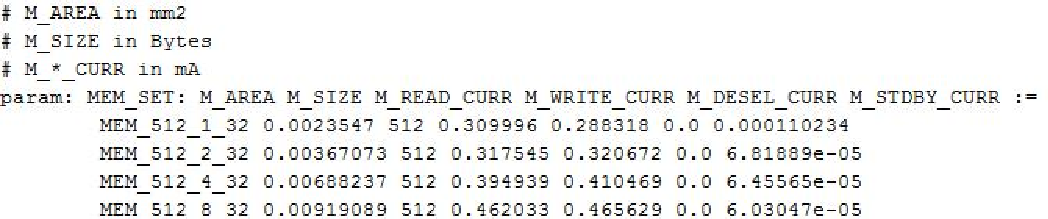
\includegraphics[width=0.7\textwidth]{mem_data}
				\label{subfig:mem_data}
			}
			\qquad
			\subfloat[][]
			{
				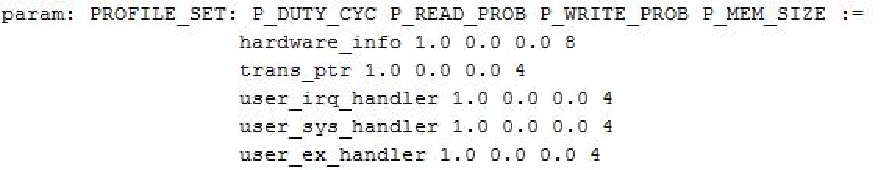
\includegraphics[width=0.7\textwidth]{profile_data}
				\label{subfig:profile_data}
			}
			\qquad
			\subfloat[][]
			{
				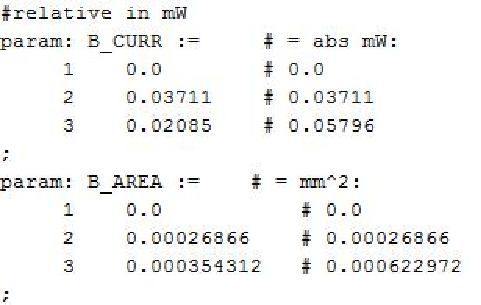
\includegraphics[width=0.4\textwidth]{ic_data}
				\label{subfig:ic_data}
			}
		\end{center}
		\caption{Fragments of The Input Parameter Data Files \cite{Strobel2016}}
		\label{fig;input_data}
	\end{figure}

	In this thesis work, the same data sets provided in \cite{Strobel2016}
	are used as the references for the input parameters data of the simulated
	annealing algorithm. These input parameters data are recorded in multiple
	plain text data files. Figure \ref{fig;input_data} represents some fragments
	of these data files. Figure \ref{subfig:mem_data} is the fragment of the
	memory data file. Figure \ref{subfig:profile_data} shows the fragment of the
	application profile data file and Figure \ref{subfig:ic_data} is the
	fragment of the interconnect data file. In order to group the data
	contained in these files into the designed input data organization, a
	parsing method is used. The basic idea of the parsing method is to read the
	plain text file line by line. The required data is extracted and the
	unnecessary data is discarded. Since the data file is text-based,
	the required data are converted into the corresponding data type during the
	extraction.

	\setlength{\textfloatsep}{0.2cm}
\begin{algorithm2e}[H]
	\KwIn{a memory\textbackslash profile data file, a memory container\textbackslash application object}
	\KwOut{void}
	\While{not end of the file}
	{
		read one line\;
		\If{relevant data is contaied in the line}
		{
			extract the data\;
			convert the extracted data into the corresponding type\;
			create a memory\textbackslash profile object based on the converted data\;
			add the created object into the list of the memroy container\textbackslash application object\;
		}
	}
	\caption{Parse Memory\textbackslash Profile Data File}
	\label{algo:mem_profile_parser}
\end{algorithm2e}
\setlength{\textfloatsep}{0.2cm}
	
	Algorithm \ref{algo:mem_profile_parser} is the pseudo-code of
	the parsing method for the memory and profile data files. If the method is
	used to parse the memory data file, it first reads one line of the file text.
	Then it checks whether there is the relevant data contained in the line or not.
	If there is no data, the the algorithm continues reading the next line.
	Otherwise, the relevant data is extracted and converted into the corresponding
	data type.
	It can be seen from the file fragment in Figure \ref{subfig:mem_data}, all the
	parameters data related to one memory type are listed in one single line.
	Thus, a memory object can be created based on the retrieved and converted data
	for one line. And the created object is added to the list in the memory container
	object. The same parsing step is repeated until the method reaches the end of
	the file. The parsing process of the application profile data file is similar
	to the parsing of the memory data file.
	The only differences are that it deals with the profile data file and the
	profile objects are created and added to the list of the application object.
	However, the parsing method of the interconnect data file is modified slightly.
	From the file fragment in Figure \ref{subfig:ic_data} it can be seen that there
	are two parts in the interconnect data file.
	The first part contains the interconnect current data while the other part
	records the interconnect area data. Thus, after the extracted data is converted,
	the parsing method needs to check whether the data is related to the current or
	the area. Then the data is added to the corresponding list of the interconnect
	object.
	
	\setlength{\textfloatsep}{0.2cm}
\begin{algorithm2e}[H]
	\KwIn{an interconnect data file, an interconnect object}
	\KwOut{void}
	\While{not end of the file}
	{
		read one line\;
		\If{relevant data is contaied in the line}
		{
			extract the data\;
			convert the extracted data into the corresponding type\;
			\eIf{is current data}
			{
				add the converted data into the current list of the interconnect object\;
			}
			{
				add the converted data into the area list in of interconnect object\;
			}
		}
	}
	\caption{Parse Interconnect Data File}
	\label{algo:ic_parser}
\end{algorithm2e}
\setlength{\textfloatsep}{0.2cm}
	
	
	
	
